\section{IoTサービス}
% (IoTサービスがどのようなもので,どのような背景で登場してきたのか,どんなものがありどのような自動化を図っているのか)}
IoTとは,Internet of Things の略で「モノのインターネット」とも呼ばれる概念である.
IoTでは,様々な物がインターネットにつながり,相互に情報をやり取りすることで,多様な自動化を行う.
IoTサービスとは,ユーザーに対しIoTによる利便性を提供するものである.
\medskip

IoTサービスは,半導体技術の進歩によりコンピューターが小型且つ安価になったこと,通信ネットワークの整備が進み様々な場所から安価に通信が利用可能になったことで登場した.
\medskip

例えば,次のような物がある.
\begin{itemize}
	\item 駐車場の検索・予約・決済サービス\cite{エコパ}
	\item 太陽光発電の監視
\end{itemize}

駐車場の検索・予約・決済サービスとは,ドライバーが空いている駐車場を探す手間を省くためのサービスである.
周囲の空いている駐車場の検索や,予め駐車場を予約しておくことで,駐車場を探す手間を省いている.
このサービスの実現のために,駐車場の駐車スペースにコンピュータを取り付ける.
これらコンピュータが,駐車場が空いているか否か・予約が入っているか否か等をサーバーとやり取りする.
それらにより,サーバーは空いている駐車場の一覧や,利用情報に基づく決済を,ユーザーに提供している.
\medskip

太陽光発電の監視とは,太陽光発電所の発電量や機器の異常を確認しに行くための手間を省くためのサービスである.
このサービスの実現の為に,太陽光発電所の機器にコンピューターを取り付ける.
これらコンピュータが発電量や機器の異常の情報をサーバーとやり取りする.
それにより,サーバーは,発電量や機器の異常をユーザーに知らせる.
\medskip

このように,IoTサービスは,IoT機器とサーバーが連携し,ユーザーに利便性を提供するものである.
今後も数多くサービスが登場すると考えられている.

\section{IoTサービスの構造}
%(IoTサービスの構造要素としてIoT機器とサーバがあること,IoT機器・サーバーとはどのようなものなのか,何をしているのか,その間の通信とはどのようなものなのか)
IoTサービスは,IoT機器とサーバーが連携し利便性を提供するものである.
IoTサービスは,多数のIoT機器とサーバーがインターネットを介し連携する構造になっている。
\medskip

\begin{figure}[htbp]
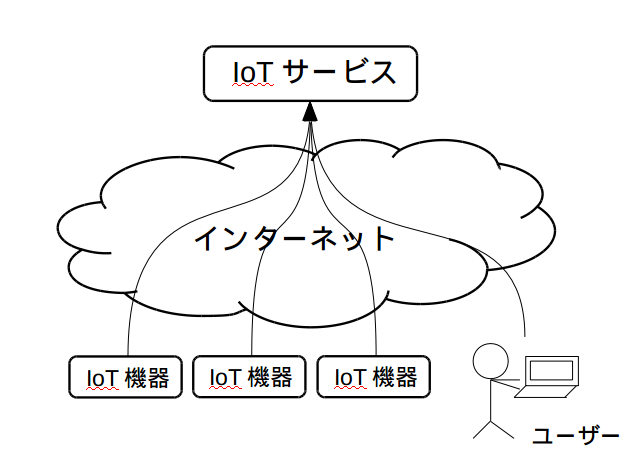
\includegraphics[width=14cm]{images/IoTservice.png}
\caption{IoTサービスの構成図}
\label{fig:IoTservice}
\end{figure}

IoT機器は,様々な環境へ設置され,周囲の状況を検知することや,周囲へなんらかの働きを行う為に使用される.
駐車場の例では,駐車スペースに車が止まっているか否かを検知している.
IoT機器の上では、サーバと情報を送受するプログラムが常時動作し、周囲の状況をサーバーに送信するか、サーバへ周囲へ何らかの働きかけを行うかどうか問い合わせている。
\medskip

この機器からの情報を収集し,処理しているのがサーバーである.
サーバーは,IoT機器からの情報を蓄積・分析し,IoT機器やユーザーに対し何らかの働きかけを行う.
駐車場の例では,駐車場の利用情報を蓄積・分析し,ユーザーへ対し可視化を行っている.
サーバーにて動作するプログラムが,IoT機器と通信することで,IoTサービスを構成する.
この通信に利用されるのがインターネットである.
様々な通信リンクを用いてIoT機器とサーバー上のプログラムが連携する.
\medskip


ユーザーは、サーバが蓄積・分析した情報を閲覧したり、サーバが蓄積・分析した情報をもととした通知を受け取る。

このように,IoTサービスの構造は,IoT機器とサーバー上のプログラムがインターネットを介し通信し,連携することで成り立っている.
図\ref{fig:IoTservice}は,IoTサービスの構造図である



\section{IoTサービスの開発・運用の問題}
%IoTサービスを開発、運用する人達として、開発者と運用者が居ることを紹介する。
IoTサービスは、IoT機器とサーバ上のプログラムがインターネットを介し通信し合うことで成り立っている。
このような構造を持つIoTサービスの開発・運用は、それぞれ異なった役割を持つ開発者と運用者が行っている。
開発者はサービスを設計・構築し、運用者は、サービスの供給が止まらないように維持・管理する役割を持っている。

%IoTサービス開発にはどのような問題があるのか説明する。
%IoTサービス開発の何がどう大変なのか、開発者の視点で説明する。
IoTサービスの開発には、次のような問題がある。
\begin{itemize}
\item 多分野に渡る技術を知っていなければならない\\
	IoT機器の開発には、ハードウェアの知識や、ネットワークの知識が必要不可欠である。
	また、サービスプログラム(?)の開発のためには、データベースやネットワークの知識が必要となる。
	このように、多分野に渡る知識を知っていなければ、開発することができない。
\item 一つの機能を実装するだけで大変\\
	IoTサービスは、一つの機能を別々の機器上で動く複数のプログラム間のやり取りにて実現するため、簡単な機能であっても、すぐに実現可能なわけではない。
\item 設置やトラブル対応が大変\\
	IoTサービスの開発には、多分野に渡る技術を知っていなければならないため、
	トラブルが発生した場合、知識のある開発者が現地に行かなければならず、コストが高い。
	また、設置の時も同様で、予め開発者が現地に行き設置環境を確認しなければならない。
\end{itemize}
このように、IoTサービスの開発は、開発者の負担が大きい。

%IoTサービスの運用にはどのような問題があるのか説明する。
%IoTサービスの運用者はどう大変なのか、説明する。(IoTサービスの構造を維持することが大変という)
IoTサービスの運用に置いては、次のような問題がある。
\begin{itemize}
\item 
\item 
\item 
\item 
\end{itemize}

このような問題から、IoTサービスの開発・運用は大変である。


%開発と運用が大変であること言うために、岡本商店街とルナネクサスさんの話をする
IoTサービスの開発と運用における要件を引き出すために、岡本商店街での実験を行った。
・実験の概要
・開発したサービスの説明
・用いた機器や開発したプログラム等の説明
 ・どのように開発したのか

また、IoTサービスを開発しているルナネクサスさんへ聞き取りを行った。
・ルナネクサスさんの説明
・ルナネクサスさんが開発しているサービスの説明
・どのような点で困っているのか、等の聞き取り結果

これらから、サービスの維持のために監視が必要であることが分かった。
また、その監視は次のような要件を満たしている必要があることが分かった。
・
・
・

\begin{comment}
%(IoTサービスの維持の為に何が必要となるのか,それを妨げている物はなんなのか)
IoTサービスは,IoT機器とサーバー上のプログラムがインターネットを介し通信し合うことで成り立っている.
IoTサービスを維持するためには,これらの構造を維持する必要がある.
そのため,IoT機器が正常に動作しているのか,通信が途切れていないか,サービスの管理者が監視する事が重要である.
ところが,IoT機器が多量に存在することや,IoT機器が接続するネットワークが多様であることから,その監視には技術的困難がある.
また,個別のIoTサービスに組み込まれた監視システム等を別として,一般的な監視サービスも存在しない.
\medskip

IoTサービスでは,多量のIoT機器を使用する.
そのため,個々のIoT機器を識別し,適切に管理することが困難である.
また,家庭内や屋外等,様々な環境下に置かれるIoT機器が接続されるネットワークを予め予期することは困難を極める.
接続先のネットワークでもプライベートアドレスを付与されるなどの他,IoT機器とサーバーとの通信に制限がかかる場合もある.
さらに,IoT機器によっては,移動することを前提とした物もある.
そのような場合,接続されるネットワークが頻繁に切り替わりるため,機器のIPアドレスを利用した既存の機器監視手法は適応することができない.
そのため,遠隔から機器の状態を確認することが難しい.
\medskip

このように,IoTサービスの維持において,IoT機器の動作や通信状態を監視することは重要であるが,その監視には技術的な困難がある.
IoTサービスの円滑な提供や今後の発展の為には,機器が設置されるネットワークに関係なく,機器が多量であっても容易に監視可能な,IoT機器の監視の実現が重要である.
\medskip

%ここから
具体的には次のような技術的困難がある。
\begin{itemize}
\item IoT機器が設置されるネットワーク環境が様々\\
	\begin{itemize}
		\item IoT機器が設置されるネットワークが、NAPTの下にある場合がある。\\
			NAPTとは、Network Address Port Transraterの事で、内側のネットワークのみで通用するIPアドレスとポート番号を必要に応じて、インターネット上で通用するIPアドレスとポート番号に変換する。
			変換の際、一時的にIPアドレスとポート番号の組み合わせを記憶し、返信があった際、記憶していたIPアドレスとポート番号の組み合わせを用いて内側のネットワークに転送する。
			そのため、内側から始まる通信は問題ないが、インターネット側から始まる通信はブロックされる。
			よって、機器監視サーバからIoT機器に対して状態を問い合わせることが出来ない。
			また、NAPT下に複数の機器が存在する場合、IPアドレスにて機器の識別をしていると、機器監視サービス側からは同一のIPアドレスからの通信に見えるので、機器が判別出来ない問題がある。
		\item IoT機器が移動する物だと、ネットワークが切り替わる場合がある。\\
			IoT機器が移動する機器である場合、ネットワークが切り替わる場合がある。
			例えば、家の中では、家に敷設されたインターネット回線を用いてインターネットへ出るが、外出先では携帯電話網を利用しているといった事があげられる。
			IPアドレスにて機器の識別をしている場合、別の機器からの通信のようにみえてしまう。
		\item セキュリティの都合上、ブロックされている場合がある。\\
			SNMPやPing等、攻撃の足がかりとなりうるプロトコルについて、ブロックされている場合がある。
			IoT機器が設置される環境によっては、機器の通信の為にブロックを解除するなどの手間が発生するが、設置される機器のネットワークが借り物である場合などは、難しい。
	\end{itemize}
\item 多量のIoT機器が存在する
	\begin{itemize}
		\item 機器監視サービスによっては、機器を追加する毎に繁雑な手順を踏まなくてはならない。
	\end{itemize}
\end{itemize}
IoTサービスの管理者が監視をしているが、監視に係る手間や監視の為に必要なことが多く困っている事を言いたい。
%ここまで

\begin{itemize}
\item IoT機器が
\item 
\item 
\item 
\end{itemize}

\end{comment}




\section{従来の機器監視手法}
\subsection{サーバからの問い合わせによる監視}
	従来から機器監視に用いられてきた手法として,定期的に機器監視サーバから対象機器に状態を問い合わせる手法がある.
	機器監視サーバから,監視対象機器上のエージェントプログラムに,現在の状態を問い合わせる事で機器の監視を実現している.
	\medskip

	代表的なものとして、次のような物がある。
	\begin{itemize}
		\item Ping\\
			Pingとは、〇〇で△△といったものである。
		\item SNMPによる問い合わせ\\
			SNMPとは、〇〇で△△といったものである。
	\end{itemize}
	
	この手法を取るメリットは、よく用いられる手法であるので、ツールなどが揃っていて手軽である点である。
	
	また、デメリットとして、次のような物がある。
	\begin{itemize}
		\item 機器は常に待ち受けていなくてはならないため、省電力を目的としたスリープをすることが難しい
		\item IPアドレスで機器を識別することになるので、NAPTの内側にある場合、機器を識別することが出来ない
		\item 攻撃の足がかりとして使われる場合もあるので、使用できない場合がある
	\end{itemize}

	IoT機器の監視は、機器がNAPTの内側にある場合が多く、ユーザーに近い場所に設置されることが多いので、この方法を用いるためには、
	機器がグローバルIPアドレスを持っていること、間のネットワークにて監視用パケットがブロックされない様ネットワーク機器を設定すること、
	が必要である。

	この形では,機器監視サーバは,監視対象機器のIPアドレスを覚えておかねばならない.
	そのため,監視対象が接続されるネットワークが切り替わった場合,監視サーバ上に記録されたIPアドレスを変更しなくては監視できない.
	監視対象が,多量且つ移動するIoT機器の監視において,頻繁に監視サーバ上に記録されたIPアドレスを書き換えるのは大変である.
	また,プライベートアドレスの利用時には,サーバーからIoT機器への到達性が失われる可能性がある.

\subsection{監視対象機器からの通知による監視}
	機器監視手法として,定期的に監視対象機器から機器監視サーバーへ状態を送信するという手法がある.
	監視対象機器上のエージェントプログラムが,指定した時間毎に機器監視サーバーへ状態を送信することで,機器の監視を実現している.
	\medskip
	
	代表的なものとして、次のようなものがある。
	\begin{itemize}
		\item SNMP Trapによる取得\\
			SNMPTrapとは先に述べたSNMPのTrapである。
		\item サーバーのリソース監視ソリューション\\
			具体的なものとして、Teregraf+Elasticsearch+Kibanaを使用したサーバー監視ソリューションがあげられる。
	\end{itemize}
	
	この手法を取るメリットは、
	1.機器から状態を送信することで、NAPTの内側に機器が設置されていても問題ない事
	2.省電力を目的としたスリープをすることができること
	がある。

	また、デメリットとして、
	1.SNMPを利用している場合は、ブロックされてしまうことがあること
	2.監視サーバの設定が繁雑であること
	がある。

	この形だと,機器監視サーバが監視対象のIPアドレスを覚えておく必要がなくなるため,監視対象が接続されるネットワークが切り替わった場合でも,追跡が可能である.
	ところが,エージェントプログラムの導入には,技術スキルと時間が必要である.
	また,サーバーの構築・設定も必要となる.

\subsection{ネットワークの提供者による機器の監視サービス} %SORACOMの話を入れる。
	ネットワーク機器から機器の監視を行うこともできる。

	代表的なものとして、株式会社SORACOMが行っているサービスが挙げられる。

	株式会社SORACOMでは、IoTプラットフォームとして、通信とクラウドを提供するサービスを行っている。
	通信はMVMOとして携帯電話網を使用しており、SORACOMAir用SIMを購入し、機器にSIMモジュールを取り付けることで利用できる。

	

	そもそも監視対象機器がつながる為のネットワークを作ってしまおうという動きもある.
	既設の携帯電話網を利用して,IoT機器用ネットワークサービスが展開されている.
	これは,IoT機器向けのデータ通信を提供するサービスで,Web画面から通信量や接続状況を確認することができる.
	携帯電話網を利用しているので,接続状況から機器の状態を推測できる.

	しかし,そのネットワークを利用している場合に限り機器の状況を推測できるので,異なるネットワークに接続された機器と,専用ネットワークを用いた機器とを1箇所で監視することが難しい.

\subsection{既存手法のまとめ}
	既存の手法として,サーバーからの問い合わせによる監視,監視対象機器からの通知による監視,ネットワークによる監視といった手法がある.
%	サーバーからの問い合わせによる監視は,現実的でなく,

\section{岡本商店街での事例}
\input okamoto.tex

\section{株式会社SORACOM様へヒアリング}
\input soracom.tex

\section{株式会社ルナネクサス様へ聞き取り}
\input lunanexus.tex






